\documentclass[a4paper]{article}
\usepackage{amsmath,amssymb,algorithmic,booktabs,bm,caption,cases,csvsimple,enumerate,float,geometry,graphicx,indentfirst,makecell,multirow,setspace,tabularx,titlesec}
\captionsetup[figure]{labelsep=period}
\captionsetup[table]{labelsep=period}
\geometry{left=3.5cm,right=3.5cm,top=3.3cm,bottom=3.3cm}
\renewcommand\thesection{\arabic{section}}
\setlength{\parindent}{2em}
\begin{document}
\begin{center}
\huge
\textbf{VE216\\Introduction to Signals and Systems\\}
\Large
\vspace{30pt}
\uppercase{Homework 1}\\
\vspace{5pt}\today\\
\vspace{5pt}
Yihua Liu 518021910998
\vspace{5pt}
\rule[-10pt]{.97\linewidth}{0.05em}
\end{center}

1.

(a) The mathematical representation for this signal is
$$x(t)=|{\sin{t}}|.$$

(b) The energy of this signal is
$$E=\int_{-\infty}^\infty|x(t)|^2\mathrm{d}t=\int_{-\infty}^{\infty}\sin^2{t}\mathrm{d}t=(\frac{t}{2}-\frac{\sin{2t}}{4})\bigg|_{-\infty}^{\infty}=\infty.$$
Since $E$ is infinite, we would like to calculate the power $P$:
$$P=\lim_{T\rightarrow\infty}{\frac{1}{2T}\int_{-T}^T|x(t)|^2\mathrm{d}t}=\lim_{T\rightarrow\infty}(\frac{1}{2}-\frac{\sin{2T}}{4T})=\frac{1}{2}.$$
Since $P$ is finite and nonzero, it is an power signal rather than energy signal.

(c) For $t\in[-\pi,0]$, $x(t)=-\sin{t}$, $y(t)=-\int_{-\infty}^t\sin{\tau}\mathrm{d}\tau=\cos{t}+1$. For $t\in[0,2\pi]$, $x(t)=\sin{t}$, $y(t)=\int_{-\infty}^t\sin{\tau}\mathrm{d}\tau=\cos{0}+1+\int_0^t\sin{\tau}\mathrm{d}\tau-\cos{t}+1=3-\cos{t}.$

Hence,
\begin{numcases}{y(t)=}
  \cos{t}+1,t\in[-\pi,0]\\
  3-\cos{t},t\in[0,\pi]
\end{numcases}
The sketch is shown below:
\begin{figure}[H]
  \begin{center}
    \includegraphics[width=0.6\textwidth]{1(c).eps}
  \end{center}
  \caption{1(c).}
\end{figure}
2.

(a) The average power is
\begin{align*}
  P&=\lim_{T\rightarrow\infty}\frac{1}{2T}\int_{-T}^T|e^{-2t}u(t)|^2\mathrm{d}t\\
  &=\lim_{T\rightarrow\infty}\frac{1}{2T}(\int_{-T}^0|e^{-2t}\cdot0|^2\mathrm{d}t+\int_0^T|e^{-2t}\cdot1|^2\mathrm{d}t)\\
  &=\lim_{T\rightarrow\infty}\frac{1}{2T}\int_0^Te^{-4t}\mathrm{d}t\\
  &=\lim_{T\rightarrow\infty}-\frac{1}{8T}(e^{-4T}-1)\\
  &=0.
\end{align*}

The energy is
$$E=\int_{-\infty}^\infty|e^{-2t}u(t)|^2\mathrm{d}t=\int_{-\infty}^{0}|e^{-2t}\cdot0|^2\mathrm{d}t+\int_{0}^{\infty}|e^{-2t}\cdot1|^2\mathrm{d}t=\int_{0}^{\infty}e^{-4t}\mathrm{d}t=\frac{1}{4}.$$

(b) Using $|e^{j(\omega_0t+\varphi)}|=1$, we have the average power is
$$P=\lim_{T\rightarrow\infty}\frac{1}{2T}\int_{-T}^T|e^{j(2t+\frac{\pi}{4})}|^2\mathrm{d}t=\lim_{T\rightarrow\infty}\frac{1}{2T}\int_{-T}^T1\mathrm{d}t=1.$$

The energy is
$$E=\int_{-\infty}^\infty|e^{j(2t+\frac{\pi}{4})}|^2\mathrm{d}t=\int_{-\infty}^{\infty}1\mathrm{d}t=\infty.$$

(c) The average power is
$$P=\lim_{T\rightarrow\infty}\frac{1}{2T}\int_{-T}^T|\cos{t}|^2\mathrm{d}t=\lim_{T\rightarrow\infty}(\frac{1}{2T}+\frac{\sin{2T}}{4T})=\frac{1}{2}.$$

The energy is
$$E=\int_{-\infty}^\infty|\cos{t}|^2\mathrm{d}t=(\frac{t}{2}+\frac{\sin{2t}}{4})\bigg|_{-\infty}^{\infty}=\infty.$$

(d) The average power is
\begin{align*}
  P=&\lim_{N\rightarrow\infty}\frac{1}{2N+1}\sum_{n=-N}^{+N}|(\frac{1}{2})^nu[n]|^2\\
  &=\lim_{N\rightarrow\infty}\frac{1}{2N+1}(\sum_{n=-N}^{-1}|(\frac{1}{2})^n\cdot0|^2+\sum_{n=0}^{+N}|(\frac{1}{2})^n\cdot1|^2)\\
  &=\lim_{N\rightarrow\infty}\frac{1}{2N+1}\sum_{n=0}^{+N}(\frac{1}{4})^n\\
  &=\lim_{N\rightarrow\infty}\frac{4}{3(2N+1)}(1-\frac{1}{4^N})\\
  &=0.
\end{align*}

The energy is
$$E=\sum_{n=-\infty}^{+\infty}|(\frac{1}{2})^nu[n]|^2=\sum_{n=-\infty}^{-1}|(\frac{1}{2})^n\cdot0|^2+\sum_{n=0}^{\infty}|(\frac{1}{2})^n\cdot1|^2=\sum_{n=0}^{\infty}(\frac{1}{4})^n=\frac{4}{3}.$$

(e) The average power is
$$P=\lim_{N\rightarrow\infty}\frac{1}{2N+1}\sum_{n=-N}^{+N}|e^{j(\frac{\pi}{2n}+\frac{pi}{8})}|^2=\lim_{N\rightarrow\infty}\frac{1}{2N+1}\sum_{n=-N}^{+N}1=1.$$

The energy is
$$E=\sum_{n=-\infty}^{+\infty}|e^{j(\frac{\pi}{2n}+\frac{\pi}{8})}|^2=\sum_{n=-\infty}^{+\infty}1=\infty.$$

(f) Since $x_3[n]=\cos{\frac{\pi}{4}n}$ is a periodic signal with the period $T=\frac{2\pi}{\omega_0}=8$, we have $\sum_{n=N}^{N+T-1}|\cos{\frac{\pi}{4}n}|=2+2\sqrt{2}$. Thus, the energy in a period is
$$E_\text{period}=\sum_{n=0}^{T-1}|\cos{\frac{\pi}{4}n}|^2=12+8\sqrt{2}$$
and the average power in a period
$$P_\text{period}=\frac{1}{T}E_\text{period}=\frac{3}{2}+\sqrt{2}.$$

Thus, the average power is
$$P=\lim_{N\rightarrow\infty}\frac{1}{2N+1}\sum_{n=-N}^{+N}|\cos{\frac{\pi}{4}n}|^2=\frac{3}{2}+\sqrt{2}.$$

The power is
$$E=\sum_{n=-\infty}^{+\infty}|\cos{\frac{\pi}{4}n}|^2=\infty.$$

3.

The average value is
$$A=\lim_{T\rightarrow\infty}\frac{1}{2T}\int_{-T}^Tx(t)\mathrm{d}t=\lim_{T\rightarrow\infty}\frac{1}{2T}(\int_{-T}^00\cdot\mathrm{d}t+\int_0^Te^{-t}\mathrm{d}t)=\lim_{T\rightarrow\infty}-\frac{e^{-T}}{2T}=0.$$

The average power is
$$P=\lim_{T\rightarrow\infty}\frac{1}{2T}\int_{-T}^T|x(t)|^2\mathrm{d}t=\lim_{T\rightarrow\infty}\frac{1}{2T}(\int_{-T}^00\cdot\mathrm{d}t+\int_0^T|e^{-t}|^2\mathrm{d}t)=\lim_{T\rightarrow\infty}-\frac{e^{-2T}}{4T}=0.$$

The energy is
$$E=\int_{-\infty}^\infty|x(t)|^2\mathrm{d}t=\int_{-\infty}^00\cdot\mathrm{d}t+\int_0^\infty|e^{-t}|^2\mathrm{d}t=\int_0^\infty e^{-2t}\mathrm{d}t=\frac{1}{2}.$$

4.

(a) A mathematical representation fot $x(t)$ is
$$x(t)=(t+2)(u(\frac{t}{2}+1)-u(\frac{t}{2}))+2(u(t)-u(t-2))+2(t-1)(u(t-1)-u(t-2)).$$

(b) To sketch $s(t)=x(-2t+1)/2$, we first do time shifting:
\begin{figure}[H]
  \begin{center}
    \includegraphics[width=0.6\textwidth]{4(b)_1.eps}
  \end{center}
  \caption{$x(t+1)=(t+3)(u(\frac{t}{2}+\frac{3}{2})-u(\frac{t}{2}+\frac{1}{2}))+2(u(t+1)-u(t-1))+2t(u(t)-u(t-1))$}
\end{figure}
and then do time scaling:
\begin{figure}[H]
  \begin{center}
    \includegraphics[width=0.6\textwidth]{4(b)_2.eps}
  \end{center}
  \caption{$x(-2t+1)=(-2t+3)(u(-t+\frac{3}{2})-u(-t+\frac{1}{2}))+2(u(-2t+1)-u(-2t-1))-4t(u(-2t)-u(-2t-1)).$}
\end{figure}
Finally, we do amplitude scaling and finally sketch $s(t)$:
\begin{figure}[H]
  \begin{center}
    \includegraphics[width=0.6\textwidth]{4(b)_3.eps}
  \end{center}
  \caption{$s(t)=x(-2t+1)/2=(-t+\frac{3}{2})(u(-t+\frac{3}{2})-u(-t+\frac{1}{2}))+(u(-2t+1)-u(-2t-1))-2t(u(-2t)-u(-2t-1)).$}
\end{figure}

(c) We can decompose $x(t)$ into its even and odd components by $x(t)=x_e(t)+x_o(t)$ where the even component is
\begin{align*}
  x_e(t)=&\frac{1}{2}[x(t)+x(-t)]\\
  &=(\frac{1}{2}t+1)(u(t+2)-u(t))+u(t)-u(t-2)+(t-1)(u(t-1)-u(t-2))\\
  &+(-\frac{1}{2}t+1)(u(-t+2)-u(-t))+u(-t)-u(-t-2)+(-t-1)(u(-t-1)-u(-t-2))
\end{align*}
and the odd component is
\begin{align*}
  x_o(t)=&\frac{1}{2}[x(t)-x(-t)]\\
  &=(\frac{1}{2}t+1)(u(t+2)-u(t))+u(t)-u(t-2)+(t-1)(u(t-1)-u(t-2))\\
  &-(-\frac{1}{2}t+1)(u(-t+2)-u(-t))-u(-t)+u(-t-2)-(-t-1)(u(-t-1)-u(-t-2)).
\end{align*}
Their sketches are shown below respectively:
\begin{figure}[H]
  \begin{center}
    \includegraphics[width=0.6\textwidth]{4(c)_1.eps}
  \end{center}
  \caption{The sketch of the even component.}
\end{figure}
\begin{figure}[H]
  \begin{center}
    \includegraphics[width=0.6\textwidth]{4(c)_2.eps}
  \end{center}
  \caption{The sketch of the odd component.}
\end{figure}
\begin{figure}[H]
  \begin{center}
    \includegraphics[width=1\textwidth]{5-6(b).jpg}
  \end{center}
\end{figure}
\begin{figure}[H]
  \begin{center}
    \includegraphics[width=1\textwidth]{6(c).jpg}
  \end{center}
\end{figure}
\begin{figure}[H]
  \begin{center}
    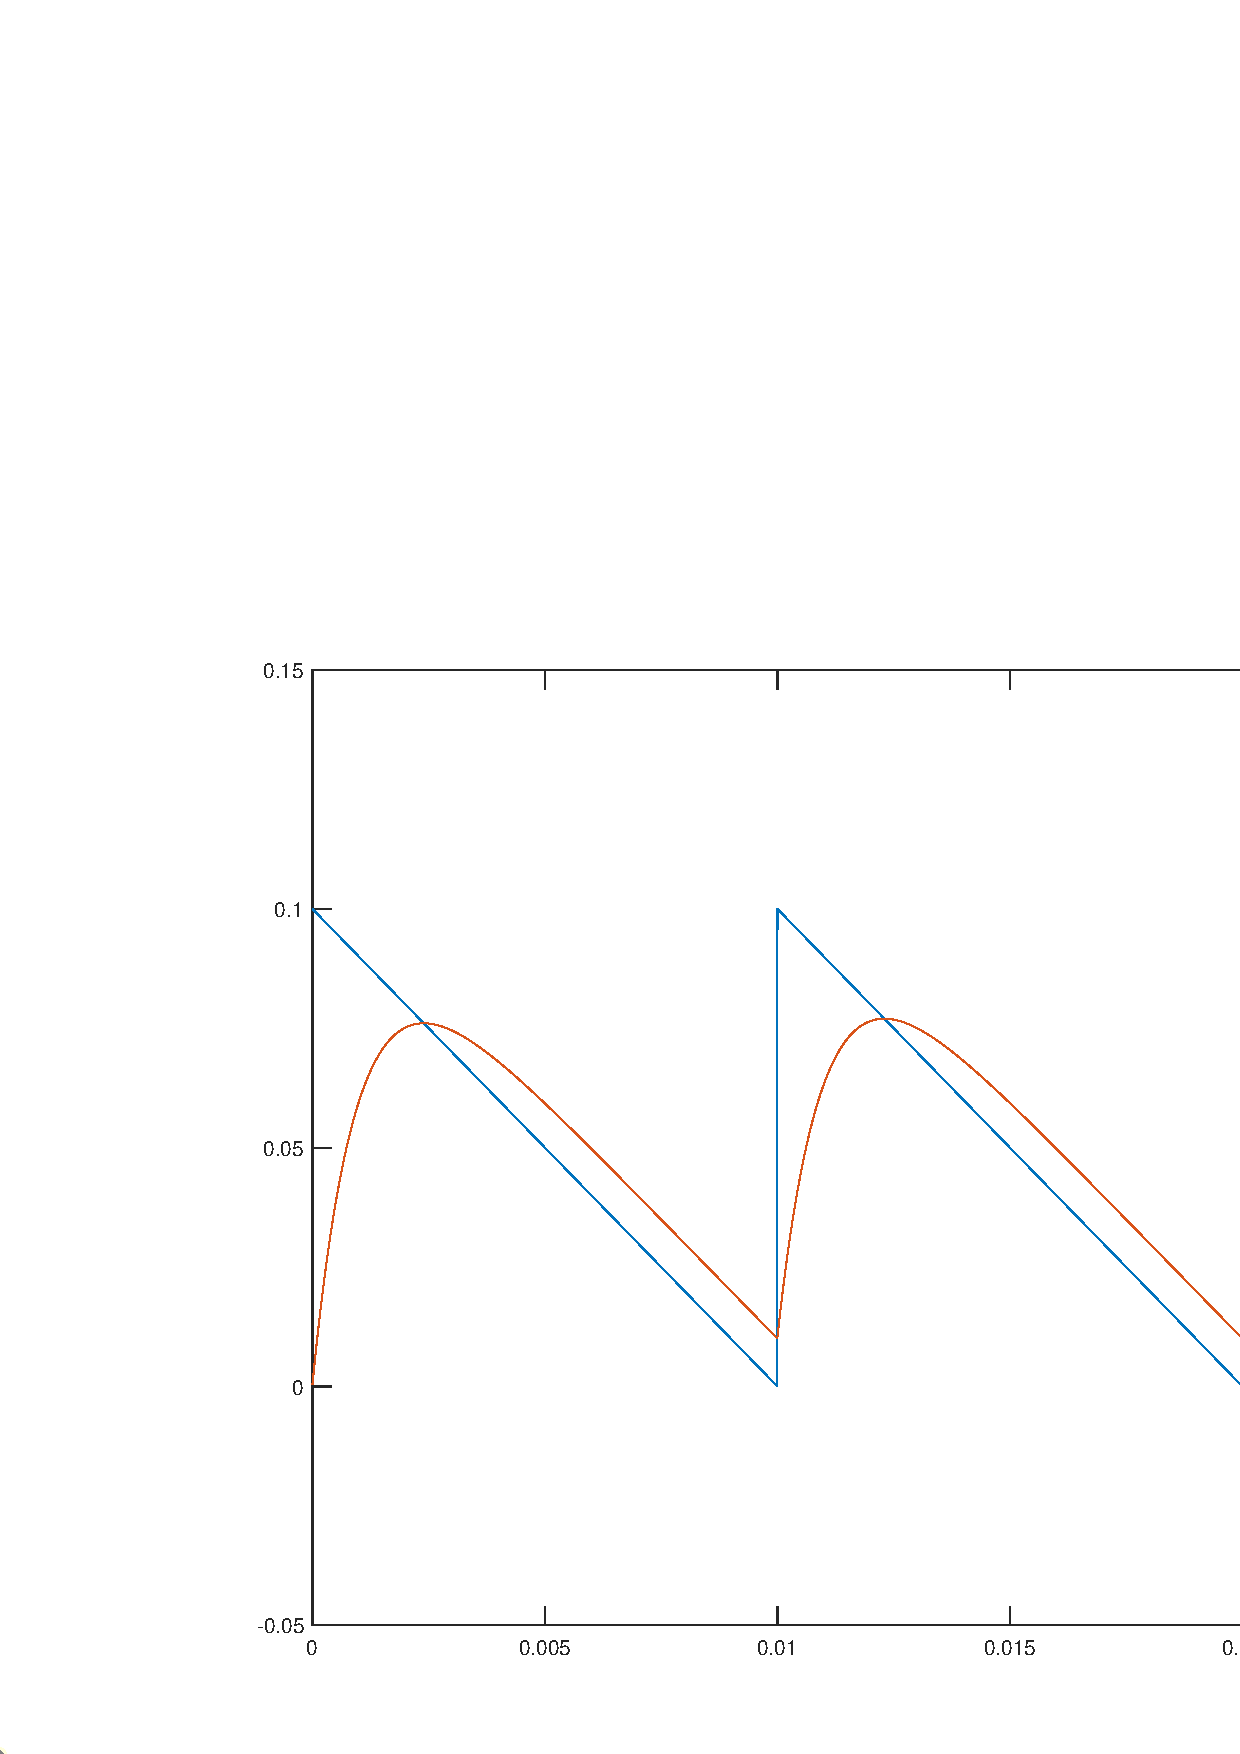
\includegraphics[width=1\textwidth]{7.jpg}
  \end{center}
\end{figure}
\newpage
8.

\begin{figure}[H]
  \begin{center}
    \includegraphics[width=0.6\textwidth]{8(a).eps}
  \end{center}
  \caption{8(a).}
\end{figure}
\begin{figure}[H]
  \begin{center}
    \includegraphics[width=0.6\textwidth]{8(b).eps}
  \end{center}
  \caption{8(b).}
\end{figure}
\begin{figure}[H]
  \begin{center}
    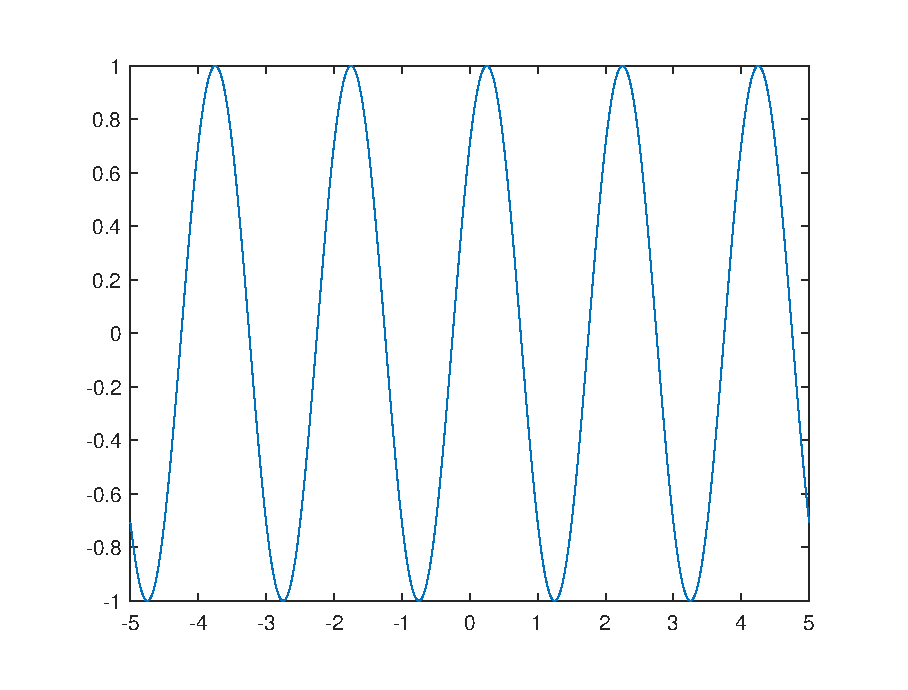
\includegraphics[width=0.6\textwidth]{8(c).eps}
  \end{center}
  \caption{8(c).}
\end{figure}
\begin{figure}[H]
  \begin{center}
    \includegraphics[width=1\textwidth]{9-11(b).jpg}
  \end{center}
\end{figure}
\begin{figure}[H]
  \begin{center}
    \includegraphics[width=1\textwidth]{11(c)-13.jpg}
  \end{center}
\end{figure}
\begin{figure}[H]
  \begin{center}
    \includegraphics[width=1\textwidth]{14-15(c).jpg}
  \end{center}
\end{figure}
\begin{figure}[H]
  \begin{center}
    \includegraphics[width=1\textwidth]{15(d)-16.jpg}
  \end{center}
\end{figure}
\begin{figure}[H]
  \begin{center}
    \includegraphics[width=1\textwidth]{17.jpg}
  \end{center}
\end{figure}
\end{document}